
\subsubsection{Reliable Optimization Depends on tractable Convex Errors used that can Guide Optimization}


Theoretically the largest possible number of constraints would be applied to optimization, because each constraint may provide additional information about the error surface, and may more rapidly exclude great volumes of the solution space. Despite this observation, except in good luck, a successful optimization recipe will not involve the use of all available fitness criterion. This makes the task of model-data fitting far from automatic, in fact human intervention is needed because, not all error signals can be informative guides. 

%\begin{itemize}
    %\item[-] Although there is a large variety of possible errors to use, its rarely a good idea to use all of these errors at once.
    
    One type of error that is an unreliable guide, is one who, by some minor aspect, contains a reference point, that is construed differently relative to each different model parameterization. In an effort to make computer code run without error, under very many different possible conditions, it is tempting to make model measurements that are not objective and unchanging between models. 
    
    A $V_{T}$ threshold my be computed as $(\frac{1}{10})\frac{dV_{M}}{dt}$.
    
    If a neuron model has a spike height below $0mV$, you may be tempted to set a spike detectors threshold as a multiple of $\mu_{V_{M}} - \sigma_{{V_{M}}}$, the mean $V_{M} -$ the standard deviation of the $V_{M}$. This would certainly detect spikes with peaks below $0mV$, and it would work for a wide variety of models too, however, the problem is that because the measurement has a dependency that is relative its self, it is less able to objectively assess waveform differences between  different models.\\
    \\
    For example spike width measurements, need to know the time when the peak of a spike occurred such that it can measure the time between $V_{T}$ and $V_{peak}$. If the method for obtaining spike time, adjusts itself to accommodate model specific differences, in the case when spike time is the same between models, some models will say a spike occured a bit later, and others a bit earlier, resulting in an unwarranted difference between measurements, which will misguide optimization. The problem can be compounded because other measurements can depend on this measurement, such as spike height, spike width, and $V_{T}$, all of these depend on the spike detection threshold. Which is now not really constant between models.\\
    \\
    Another cause of misguided errors may involve the recalculating the Rheobase current injection value between different models, there is some error associated with approximating the rheobase current. What is desired is to ascertain the minimal current injection amplitude, which would cause only one spike to fire, but because there is not much time to exhaustively test smaller and smaller values of current amplitude (due to the exploration, exploitation dilemma), one will always settle for an over estimate, one that is somewhere between enough current to cause one or two spikes. The size of this error will vary between models. In addition to this finite precision error, a measurement that is relative to each model, and not objective between models, is a bad idea for the same reason as the model specific measurement for $V_{T}$.\\
    \\
    Spike amplitude will be bigger for some models at their rheobase calculation than other models, especially between models of different input Resistance. Input Resistance will succeed in attenuating greater amplitudes of applied current, however, if a the current succeeds at provoking a spike, the voltage deflection will have a larger peak because of Ohms law: $V=IR$. In this case $V_{M}$, specifically the peak of $V_{M}$ deflection is proportionate to current injection amplitude. So models with different amounts of input resistance will also differ in the peak of the rheobase current injection. However because rheobase is re-calculated per model and because there is finite precision in the rheobase error calculating software it is possible that there will be small regions of error surface, that less accurately encode this relationship.\\
    \\ 
    The situation then compounds when other measurements are taken which depend on rheobase values. An alternative exists where, you sample an error surface using a fixed amount of current preferably at the observed Rheobase current of an experimental cell you are investigating. This would make "Rheobase" a hard constraint, models either spike at the prescribed current, or they don't. Meaning many models are instantly eliminated only because they failed to match Rheobase value, and models that pass this Rheobase test, may score poorly across every other NeuronUnit criteria.
    
    The appeal of applying rheobase as a soft constraint, is it better solutions should be possible, if models are allowed to perform badly on the rheobase score and good at all other criteria, however, there may be other ways of achieving this.
    
    When applying a fixed rheobase current across many different models only neurons that fail to spike need to be excluded, neurons that fire multiple spikes can still have their spike shapes measured. Additionally, it would be acceptable to run different optimization batches, at different current injection amplitudes, and to federate scores between batches of different current amplitude. The reason why batches need to remain seperate, is that, its only important that error surfaces are convex within the one optimization process. Its okay if two different processes are using different surfaces, as each is blind to the others internal error surface.\\ 
    \\
    %The down side to this approach, is that by distributing the optimization job into batches, it begins to take on an exhaustive nature, and it is not really known, how many current levels would need to be independently explored to achieve good results.\\
    \\
    A different approach was also utilized, where three static quantities of current amplitude $(300pA, 450pA, and 900pA)$ was applied uniformly to all sampled model parameterizations. 
    Another approach, was explored were larger volumes of the solution space were immediately excluded, by way of fixed current.
    %more exclusively
    be to apply a large enough current to invoke spiking in most neurons, and to measure the wave form shape of just one or two spikes in a the resulting spike train.
    
    \subsubsection{Error signals derived from threshold calculations}
    %\begin{itemize}
    %\item[-] 
    A suite of NeuronUnit tests contained two threshold dependent measurements. These were spike half-width, spike height. The treshold was also used to comprize a NU test, so in total three $V_{T}$ measurements were used.
    
    %\item[-] 
    (Ephysiology Feature Extraction Library \cite{}) EFEL, Allen SDK, and Druckman all contain independently written algorithms for ascertaining modelled neuron $V_{T}$ thresholds calculation code. In all three feature extraction pipelines $V_{T}$ is computed by taking derivative of $V_{M}$
    %\end{itemize}
    
   Another related pitfall is the relationship between the number of free dimensions in the optimization problem versus the number of reliable errors used to constrain the optimization process.
   
   Genetic algorithms are known as derivative free optimizers, since the derivative of the error surface is not explicitly calculated, and genetic algorithms have properties that make them robust against local minima. However, just like in gradient descent, genetic algorithms act on information in the error surface. Although genetic algorithms are resilient against local minima, but they are still misguided by unfortunately positioned local error wells. For this reason Rastrigrins function is used to benchmark the performance of genetic algorithms.\\
   \\
   Rastrigins function has convexity in two scales. On the larger scale the surface has a convex property, on the small scale the function is uniformly pocked with minima wells. Inorder for the GA to optimize Rastrigins function it must be able to exploit the global information of the error surface, and simultaneously the genes will often converge for generations in the minima, but they won't get stuck there because mutation and cross-over will drive the GA to test other less optimal solutions.\\
   \\
   \begin{figure}
  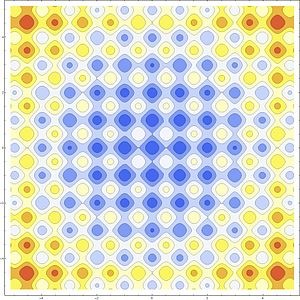
\includegraphics[]{figures/rastagrind.jpg}
  \caption{}
   \end{figure}
   
   It is worth noting that although Rastrigrins function is challenging it does not the present the worst gradient to learn from. Worse than Rastrigrins function, are functions that on a large scale are flat, but on the smaller scale contain a high density ripples.
   but lacks this global convex trend, excepting for an abrupt and localised descent to the optima.\\ 
   \\
   Without some first prior knowledge of the error surface, a likely outcome is to attempt optimize on uninformative surfaces. If an uninformative surface is applied, it does not mean that the genetic algorithm will not succeed, it only means that the performance of the GA may be only marginally better than random sampling, or exhaustive search of the error surface.\\
   \\
   Random sampling, sounds bad, however, if the best random solution is digitally stored, and the number of samples applied is less than the possible number of samples in an exhaustive search, random sampling may better resolve the exploitation/exploration dilemna than both gradient descent, and exhaustive search.
      \begin{figure}

   
\includegraphics[]{figures/pond_ripple_surface.png}
     \caption{In the case of pond ripples the cost function is defined so that the maxima is the optimal location on the surface. Ripples on a body of water are more challenging to optimize, as the water surfaces are approxmiately flat on the large scale, yet on the small scale maximas will be temporary preoccupy the GAs learning, but outside of those peaks, there is little large scale information to utilize. }

      \end{figure}

   
   When considering 2D relationships between single parameters and single objective functions, ideally each objective function might contribute helpful information, that on mass boosts the total amount of helpful information. For-instance some 2D error mappings, may contain one or more local minima, but in the same region a different error mapping could lack the well, meaning that at least one out of two error functions contribute incentive to stride across a minima. The mapping that contains wells, might still be useful to guide optimization, as it may also lack minima in regions were the counterpart has them, additionally the counterpart mapping may have regions of $~0.0$ gradient where the other mapping contains significant gradient.\\
   \\
   It is almost impossible to make progress without some prior knowledge of the error surfaces, as knowledge of the error surface is a prerequisite for constraining optimization. Not all surfaces, provide equally useful information. There are spectrums of surface quality between convex traingular or parabolic depressions acting as the best solution surfaces, and flat functions 
   $NDIM:NOBJ$
   
   Ideally each extra $NOBJ$  

%\end{itemize}